%&"../main"
\documentclass[../main]{subfiles}
\begin{document}

\chapter{通用DSP实现FIR滤波器}%
\label{cha:通用DSP实现FIR滤波器}

\section{实验目的}%
\label{sec:\arabic{chapter}实验目的}

\begin{enumerate}

	\item 了解FIR滤波器的DSP实现方法;

	\item 了解用FIR滤波器实现模拟信号滤波的全过程;

	\item 掌握FIR滤波器直接型结构的实现方法。

\end{enumerate}

\section{实验原理}%
\label{sec:\arabic{chapter}实验原理}

FIR滤波器是有限长单位脉冲响应数字滤波器,其系统函数一般式为:

\begin{align}
	H(z) = \sum\limits_{n=0}^{N-1}h\left[n\right]z^{-n}
\end{align}

FIR滤波器的通用DSP实现法与前面介绍的IIR滤波器结构的实现方法类似, 用FIR滤波器对模
拟信号进行滤波的结构图\ref{fig:数字滤波器对模拟信号滤波的原理图}所示。

\begin{figure}[htbp]
	\centering
	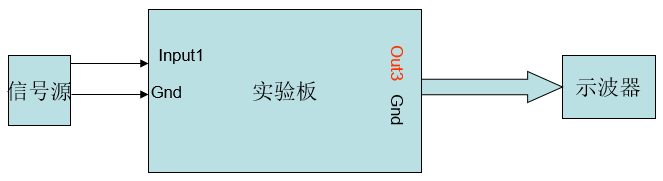
\includegraphics[width = 0.8\linewidth]{dia.png}
	\caption{数字滤波器对模拟信号滤波的原理图}
	\label{fig:数字滤波器对模拟信号滤波的原理图}
\end{figure}

本实验中在以通用DSP(TMS320)为核心的DSP平台上采用窗函数设计法分别设计了50阶的高通
、低通、带通FIR滤波器,其幅频特性分别如图\ref{fig:FIR频响特性}所示:

\begin{figure}[htbp]
	\centering
	\begin{subfigure}[htbp]{.45\linewidth}
		\centering
		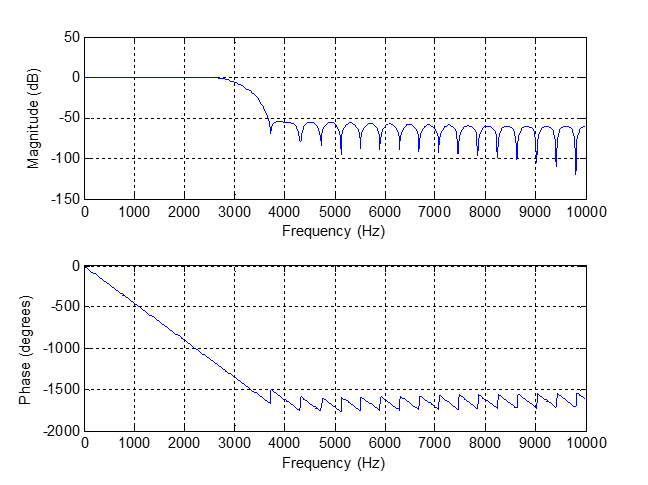
\includegraphics[width = \linewidth]{LP.png}
		\caption{LPFIR}
		\label{fig:LPFIR}
	\end{subfigure}
	\quad
	\begin{subfigure}[htbp]{.45\linewidth}
		\centering
		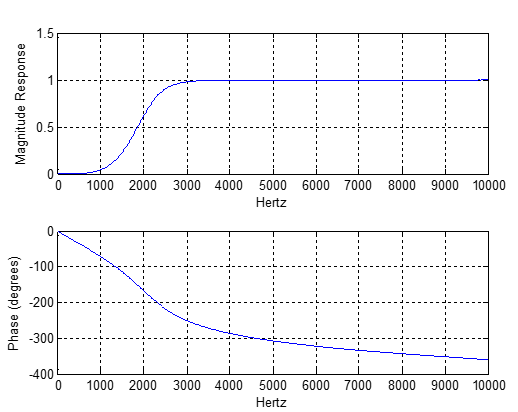
\includegraphics[width = \linewidth]{HP.png}
		\caption{HPFIR}
		\label{fig:HPFIR}
	\end{subfigure}

	\begin{subfigure}[htbp]{.45\linewidth}
		\centering
		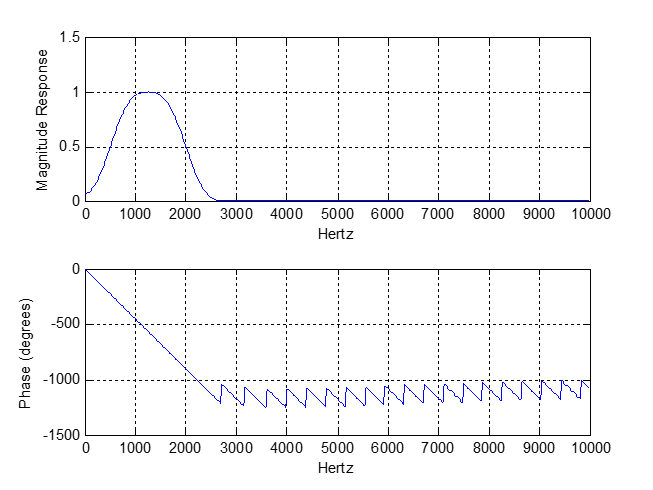
\includegraphics[width = \linewidth]{BP.png}
		\caption{BPFIR}
		\label{fig:BPFIR}
	\end{subfigure}
	\caption{FIR频响特性}
	\label{fig:FIR频响特性}
\end{figure}

\section{实验仪器、仪表}%
\label{sec:\arabic{chapter}实验仪器、仪表}

\begin{table}[htbp]
	\centering
	\caption{实验仪器、仪表}
	\label{tab:实验仪器、仪表}
	\csvautobooktabular{tab/BOM.csv}
\end{table}

\section{实验预习要求}%
\label{sec:\arabic{chapter}实验预习要求}

认真复习采样定理、IIR滤波器的结构以及A/D 、D/A转换器等有关内容,阅读TMS320F2812的
有关知识及实验原理、实验所用其它器件的性能和使用方法。

\section{实验原理图}%
\label{sec:\arabic{chapter}实验原理图}

\begin{figure}[htbp]
	\centering
	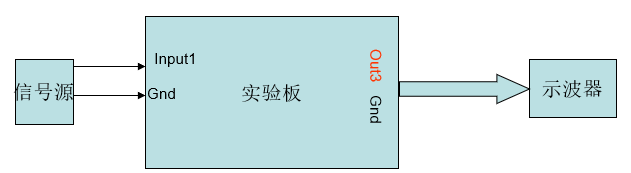
\includegraphics[width = 0.8\linewidth]{scheme.png}
	\caption{实验原理图}
	\label{fig:实验原理图}
\end{figure}

\section{实验内容及步骤}%
\label{sec:\arabic{chapter}实验内容及步骤}

\begin{enumerate}

	\item 按实验连接图检查连线是否正确,然后依次打开信号源、示波器、实验装置的电源开关;

	\item 将信号源的频率调至50Hz,$ V_\mathrm{pp}$调至500mV,按试验箱上的提示选择1($ f_\mathrm{s} = $20kHz),再选择
		1(fir),然后选择1(低通:$ \omega_n = $0.3);

	\item 观察示波器上的输出信号。将信号源的频率从50Hz逐渐提高,观察示波器上的输出信号幅度
		的变化规律并作记录(记录点数不得少于10点),记下系统的fc ;

	\item 低通数据测量结束后,按6返回,选择1($ f_\mathrm{s} = $20kHz),再选择1(fir),然后选择3(带通:ω
		n=0.05~0.2);

	\item 重复步骤3的操作,测量带通滤波器的频响特性;

	\item 带通数据测量结束后,按6返回,选择2($ f_\mathrm{s} = $27.9kHz),再选1(fir)择,然后再选择1(低通:$ \omega_n = $0.3);

	\item 重复步骤3的操作,测量不同采样频率下高通滤波器的频响特性;

	\item 高通数据测量结束后,按6返回,选择2($ f_\mathrm{s} = $27.9kHz),再选择1(fir),然后再选择3(带通:$ \omega_n = $0.05--0.2);

	\item 重复步骤3的操作,测量不同采样频率下带通滤波器的频响特性。

\end{enumerate}

\section{实验报告}%
\label{sec:\arabic{chapter}实验报告}

\begin{Exercise}

	写明实验目的、实验原理、实验内容及步骤;

\end{Exercise}

\begin{Answer}

	实验目的见章节\ref{sec:\arabic{chapter}实验目的},实验原理见章节
	\ref{sec:\arabic{chapter}实验原理},实验内容及步骤见章节
	\ref{sec:\arabic{chapter}实验内容及步骤}。

\end{Answer}

\begin{Exercise}

	整理实验数据,在坐标纸上分别画出所测系统的频响特性曲线,比较所测各种滤波器
	带宽与理论带宽的误差;并比较相同$ \omega_n $、不同采样频率下实验所得同种
	滤波器的带宽,得出滤波器带宽与采样频率之间的关系。

\end{Exercise}

\begin{Answer}

	频响特性曲线见图\ref{fig:FIR}。比较图\ref{fig:FIR频响特性}和
	\ref{fig:FIR},可见实验数据与仿真结果比较吻合。数字信号的带宽与采样率成
	正比例关系。

\end{Answer}

\begin{figure}[htbp]
	\centering
	\begin{subfigure}[htbp]{.45\linewidth}
		\centering
		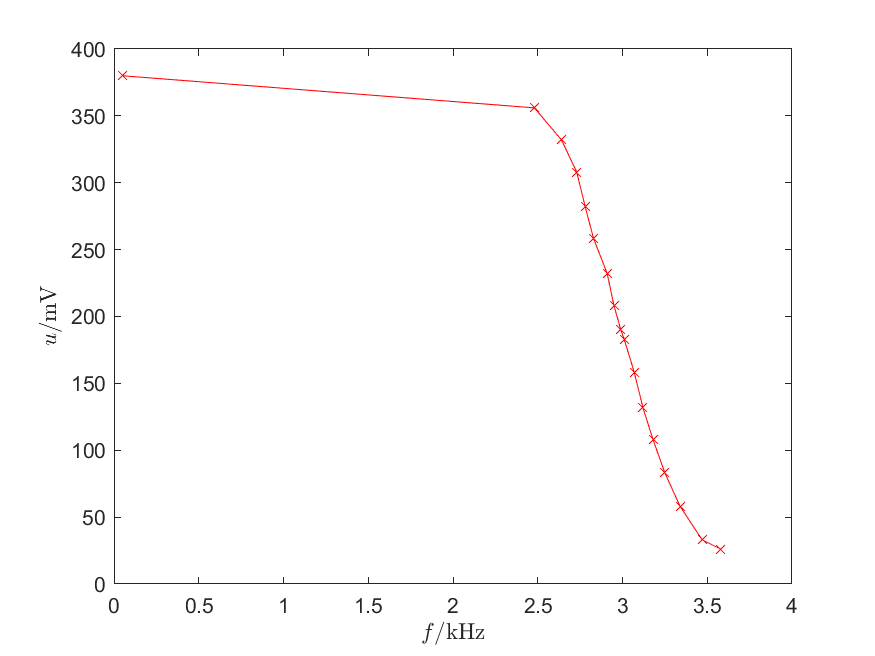
\includegraphics[width = \linewidth]{LPFIR20.png}
		\caption{LPFIR20kHz}
		\label{fig:LPFIR20}
	\end{subfigure}
	\quad
	\begin{subfigure}[htbp]{.45\linewidth}
		\centering
		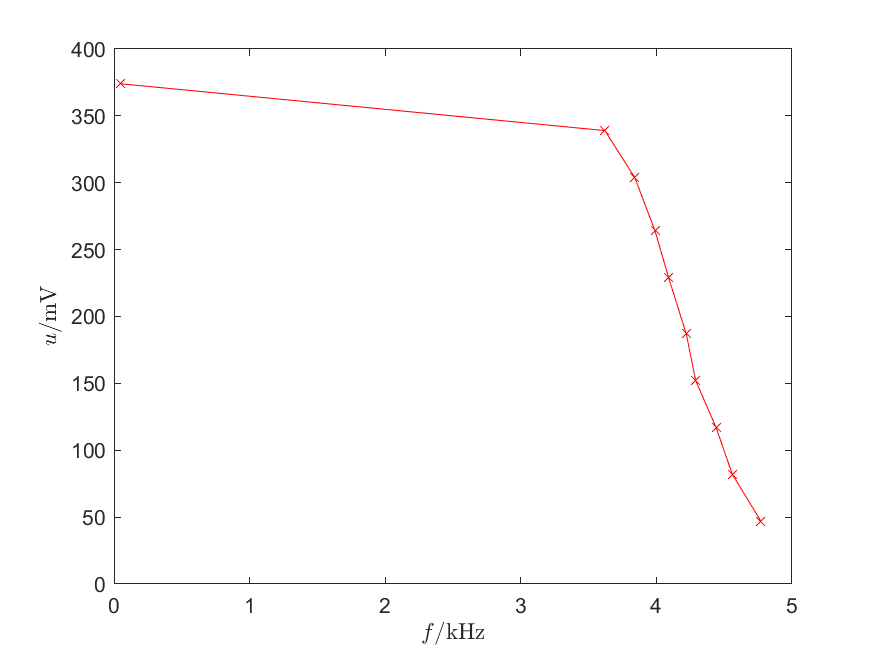
\includegraphics[width = \linewidth]{LPFIR27.png}
		\caption{LPFIR27.9kHz}
		\label{fig:LPFIR27}
	\end{subfigure}

	\begin{subfigure}[htbp]{.45\linewidth}
		\centering
		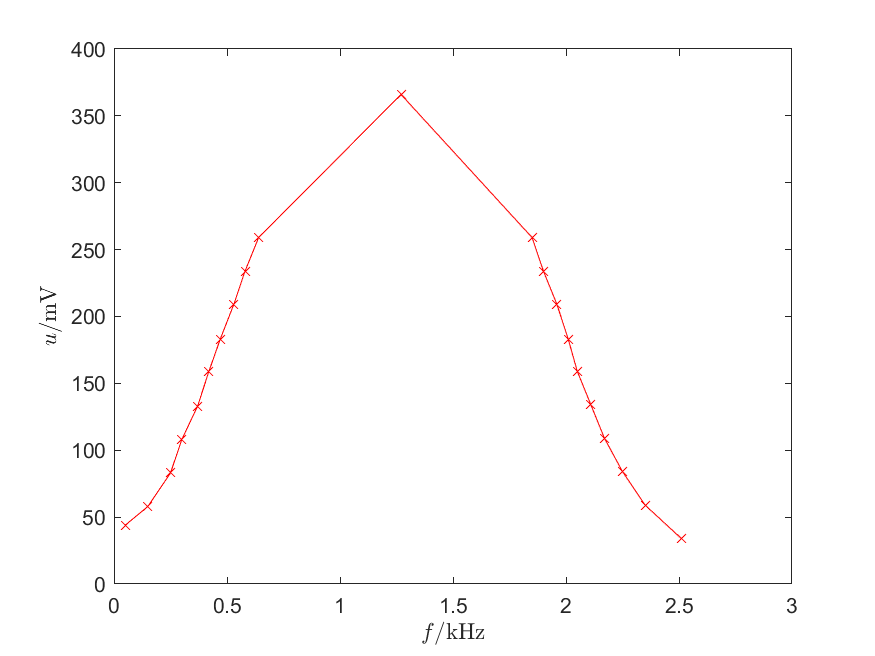
\includegraphics[width = \linewidth]{BPFIR20.png}
		\caption{BPFIR20kHz}
		\label{fig:BPFIR20}
	\end{subfigure}
	\quad
	\begin{subfigure}[htbp]{.45\linewidth}
		\centering
		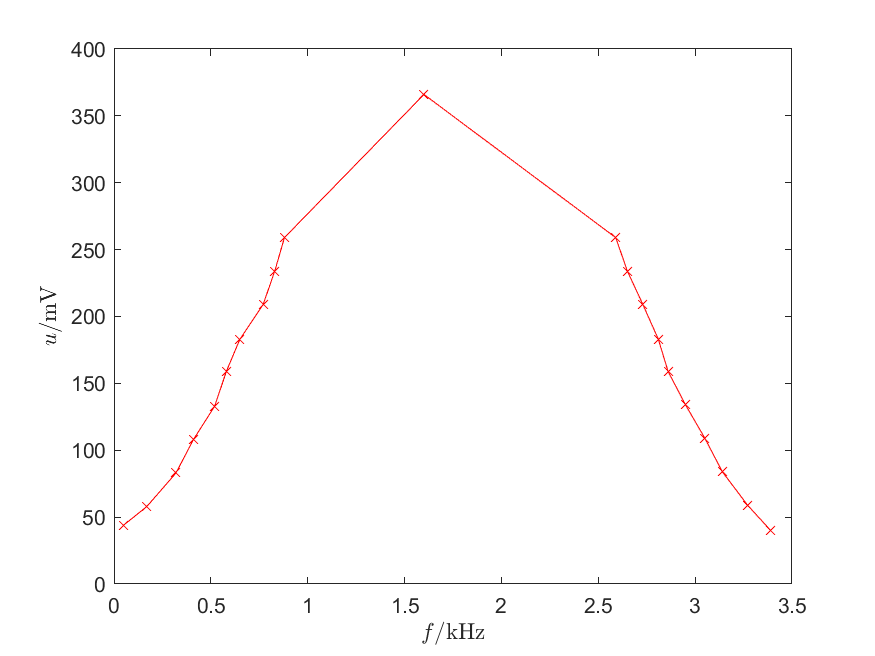
\includegraphics[width = \linewidth]{BPFIR27.png}
		\caption{BPFIR27.9kHz}
		\label{fig:BPFIR27}
	\end{subfigure}
	\caption{FIR}
	\label{fig:FIR}
\end{figure}

\begin{table}[htbp]
	\centering
	\caption{LPFIR20kHz}
	\label{tab:LPFIR20kHz}
	\csvautobooktabular{tab/LPFIR20.csv}
\end{table}

\begin{table}[htbp]
	\centering
	\caption{LPFIR27.9kHz}
	\label{tab:LPFIR27.9kHz}
	\csvautobooktabular{tab/LPFIR27.csv}
\end{table}

\begin{table}[htbp]
	\centering
	\caption{BPFIR20kHz}
	\label{tab:BPFIR20kHz}
	\csvautobooktabular{tab/BPFIR20.csv}
\end{table}

\begin{table}[htbp]
	\centering
	\caption{BPFIR27.9kHz}
	\label{tab:BPFIR27.9kHz}
	\csvautobooktabular{tab/BPFIR27.csv}
\end{table}

\end{document}

